\documentclass{beamer}
\mode<presentation> {
    \usetheme{Copenhagen} \usecolortheme{whale}
    }
\usepackage{graphicx}
\usepackage{multicol}
\usepackage{subfig}

\setbeamersize{text margin left=3mm,text margin right=5mm }
\geometry{paperwidth=500pt, paperheight=300pt}
\usepackage{verbatim}
\graphicspath{{Images/}}
\title[Assignments 6]{Robust Stability and Robust Performance}
\author{Lorenzo Rossi Matricola: 0301285}
\begin{document}
\begin{frame}
	\titlepage{}
\end{frame}
\begin{frame}
	\begin{columns}[t]
		\begin{column}{.5\textwidth}
			\tableofcontents[sections={1-3}] % chktex 8
		\end{column}
		\hspace{-1cm}
		\begin{column}{.5\textwidth}
			\tableofcontents[sections={4-5}] % chktex 8
		\end{column}
	\end{columns}
\end{frame}
\begin{frame}
	\frametitle{Assignment 6}
	\section{Introduzione}
	Consideriamo la famiglia degli impianti:\begin{equation}
		\tilde{P}= P(1+\Delta W_{2})
	\end{equation}
	con \(P(s)=\frac{1}{s-1},\quad W_{2}(s)=\frac{2}{s+10},\quad C(s)=k,\quad W_{1}(s)=\frac{1}{s+1}\). Assumendo che \(\Delta \) è tale che \(\left\lVert \Delta\right\rVert_{\infty }\leq 2\), determinare l'intervallo dei valori di \(k\) per cui si otteniene la stabilità robusta e determinare il valori di \(k\) per per cui si ottiene stabilità rousta e minimizza le prestazioni robuste di lvello \(\alpha \).
\end{frame}
\begin{frame}
	\frametitle{Stabilità Robusta}% chktex 8
	\section{Stabilità Robusta}
	\(\Delta \) è una incertezza di livello \(\beta = 2\). Quindi, la condizione di stabilità robusta è data da \(\left\lVert W_{2}T\right\rVert_{\infty}<\frac{1}{\beta}=\frac{1}{2}\) dato che, utilizzando il teorema del piccolo guadagno e separando il sistema a ciclo chiuso dall'incertezza, si ottiene che:
	\begin{align*}
		\Delta_{in}\rightarrow \Delta_{out}: & W_{2}\frac{PC}{1+PC}=W_{2}\frac{L}{1+L}=W_{2}T                                                                                                                                                                                                        \\
		\text{Deve valere che:}                                                                                                                                                                                                                                                                      \\
		                                     & \left\lVert \Delta\right\rVert_{\infty}\left\lVert W_{2}T\right\rVert_{\infty}<1\longrightarrow^{\left\lVert \Delta\right\rVert_{\infty}\leq 2} 2\cdot\left\lVert W_{2}T\right\rVert_{\infty}<1\rightarrow \left\lVert W_{2}T\right\rVert<\frac{1}{2}
	\end{align*}
	Preliminarmente, occorre rispettare la stabilità del sistema a ciclo chiuso. A tale scopo, si considera il luogo delle radici di\(L=PC\) da cui si ottiene il seguente risultato.

\end{frame}

\begin{frame}
	\frametitle{Stabilità Robusta}
	\begin{figure}
		\centering
		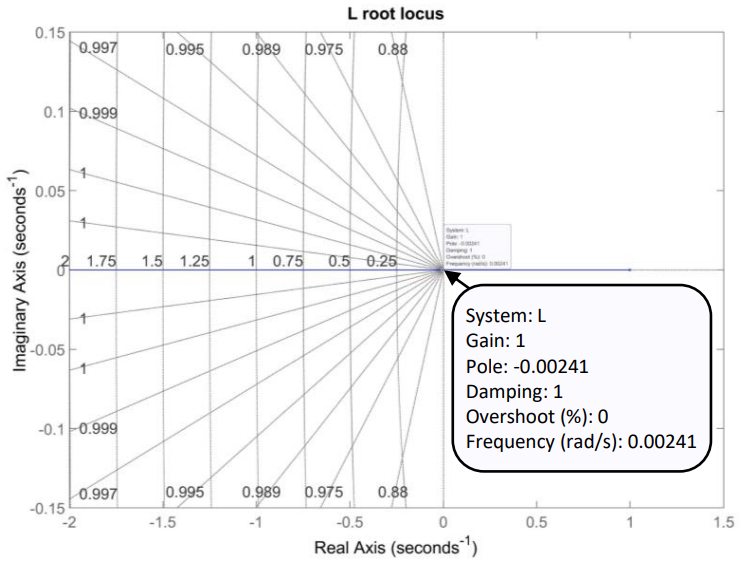
\includegraphics[scale=0.4]{2022-06-09-16-12-21.png}% chktex 8
	\end{figure}
	Quindi, si ha stabilità asintotica nominale per \(k>1\). Un metodo alternativo può essere dato dall'analisi dei poli della funzione di sensitività \(S=\frac{1}{1+L}=\frac{1}{1+PC}=\frac{s-1}{s-1+k}\).
\end{frame}
\begin{frame}
	\frametitle{Stabilità Robusta}
	\footnotesize
	\begin{minipage}{0.45\textwidth}
		Considerando esplicitamente il diagramma dei moduli di:
		\begin{align*}
			W_{2}T = W_{2}\frac{2k}{1+PC}=\frac{2k}{s^{2}+s(9+k)+10(k-1)}
		\end{align*}
		Si ottiene che il guadagno maggiore si ottiene per \(\omega = 0\):
		\begin{equation*}
			\left\lVert W_{2}T\right\rVert_{\infty}=|W_{2}T|_{\omega =0}= \frac{2k}{10(k-1)}=\frac{k}{5k-5}
		\end{equation*}
		Per avere stabilità robusta dobbiamo soddisfatte:\begin{equation*}
			\frac{k}{5(k-1)}<\frac{1}{2}\rightarrow k>\frac{5}{3}
		\end{equation*}
		Inoltre, per \(k=1\), il sistema risulta instabile poiché il diagramma di Nyquist passa per il punto \(-1+0j\). Con l'aumentare di \(k\) aumenta la distanza dal punto \(-1+0j\) e per \( k>\frac{5}{3}\) si soddisfano le specifiche di robustezza.
	\end{minipage}\hspace{1cm}
	\begin{minipage}{0.45\textwidth}
		\begin{figure}
			\centering
			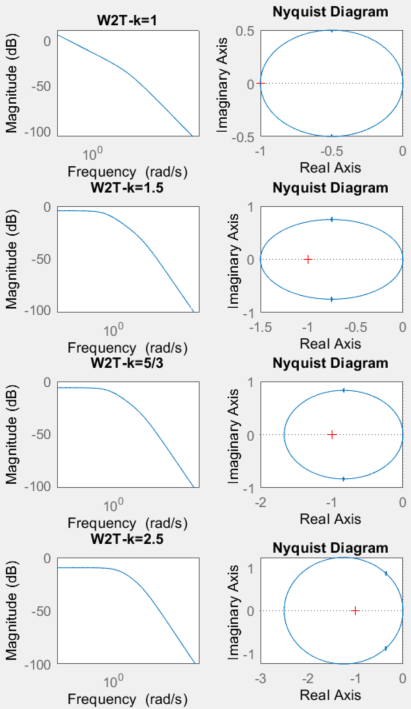
\includegraphics[width=150pt,height=200pt]{2022-06-09-16-40-44.png}% chktex 8
		\end{figure}
	\end{minipage}

\end{frame}
\begin{frame}
	\frametitle{Stabilità Robusta e Prestazioni Robuste}
	\section{Stabilità Robusta e Prestazioni Robuste}
	Per garantire prestazioni robuste di livello \(\alpha \) e tollerare incertezze di livello \(\beta =2 \), devono essere soddisfatte:
	\begin{equation*}
		\left\lVert W_{2}T\right\rVert_{\infty}<\frac{1}{2}\quad \land  \left\lVert W_{1}\tilde{S}\right\rVert_{\infty}=\left\lVert \frac{W_{1}S}{1+\Delta W_{2}T}\right\rVert<\alpha\quad \forall\Delta:\left\lVert \Delta\right\rVert_{\infty}\leq 2
	\end{equation*}
	\begin{align*}
		 & \max_{\left\lvert \Delta\right\rvert\leq 2}\left\lvert \frac{W_{1}S}{1+\Delta W_{2}T}\right\rvert=\frac{\left\lvert W_{1}S \right\rvert}{1-2 \left\lvert W_{2}T\right\rvert}<\alpha \Rightarrow \alpha_{\min}=\max_{\omega}{\frac{\left\lvert W_{1}S \right\rvert}{1-2 \left\lvert W_{2}T\right\rvert}}=\left\lVert \frac{\left\lvert W_{1}S \right\rvert}{1-2 \left\lvert W_{2}T\right\rvert}\right\rVert_{\infty} \\
		 & W_{1}S=\frac{s-1}{s^{2}+ks+k-1}\quad \text{massimo in }\omega=0                                                                                                                                                                                                                                                                                                                                                     \\
		 & \left\lvert W_{1}S(0)\right\rvert =\frac{1}{k-1}\Rightarrow \alpha_{\min}=\frac{5}{3k-5}\rightarrow k>\frac{5}{3}
	\end{align*}
\end{frame}

\begin{frame}
\frametitle{Stabilità Robusta e Prestazioni Robuste}
\begin{minipage}{0.33\textwidth}
	Ne deriva quindi che:\begin{itemize}
		\item il più grande valore di \(k \) è il più piccolo valore di \(\alpha \) raggiungibile;
		\item Con l'aumentare di \(k \) si ha che \(\left\lVert W_{2}T\right\rVert_{\infty}\) e \(\left\lVert W_{1}S\right\rVert_{\infty} \) diventano sempre più piccoli;
		\item Il diagramma polare di \(L \) per \(k>\frac{5}{3}\) si allontana sempre di più dal punto \(-1+0j \).
	\end{itemize}
\end{minipage}
\begin{minipage}{0.66\textwidth}
\begin{figure}
	\centering
		\begin{minipage}{0.49\textwidth}
			{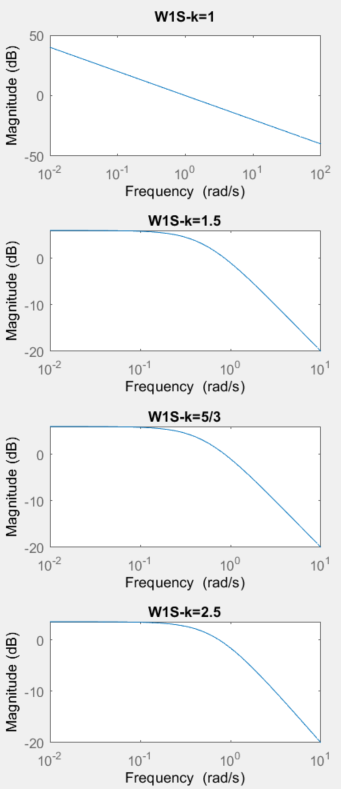
\includegraphics[scale=0.3]{2022-06-09-17-38-00.png}}% chktex 8
		\end{minipage}\hspace{-1cm}
		\begin{minipage}{0.49\textwidth}
			{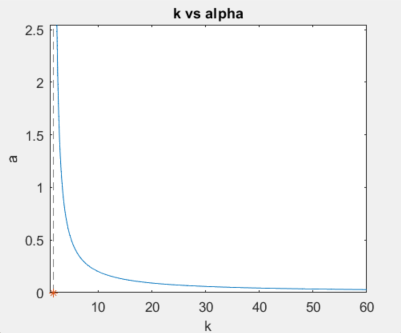
\includegraphics[scale=0.3]{2022-06-09-17-31-10.png}}% chktex 8
		\end{minipage}
\end{figure}
\end{minipage}
\end{frame}

\end{document}